\documentclass[report.tex]{subfiles}
\begin{document}

This first chapter presents the theoretical foundation for the thesis.
The theory is grouped in four categories: \gls{NN}s, learning,
neuromorphic hardware, \index{neuromorphic} and finally
the cognitive theory of the Reorganisation of Elementary Functions
(\gls{REF}).

%TODO : Add section on terminology: population in layers in networks

\section{Neural networks} \label{sec:nn}
\Gls{NN}s is a broad term that originates in the neuronal models from
biological brain \cite{Dayan2001}.
The general architecture of neural systems can be explained as circuits
of neurons \index{neuron} connected through weighted edges.
\cite{Russel2007, Dayan2001}.
In this abstract sense a neuron is defined as a computational unit that
takes a number of signals (inputs) and processes them through some
function $f$ that outputs a single value \cite{Eliasmith2004}.
From that perspective neural networks simply \textit{computes} an 
output based on some input why neural networks can be understood as
complex non-linear computations \cite{Eliasmith2004, Dayan2001}.

In a more concrete sense neural networks computes over either
continuous (e. g. voltage and numbers) or discrete signal, and they
can be modelled with or without a temporal dimension
\cite{Eliasmith2004, Russel2007, Schmidhuber2014}.

Discrete models without a temporal dimension were the foundation for
the first generation of neural networks \cite{Russel2007, Maass1997}.
They are based on the perceptron model as seen in equation
\ref{eq:perceptron}, also known as the McCulluch-Pitts neuron model
\cite{Eliasmith2004}.

\begin{equation} \label{eq:perceptron}
f(x) = \begin{cases}
	 1 & \text{if } u > 0\\
	 0 & \text{otherwise}
       \end{cases}
\end{equation}

\subsection{Second generation neural networks}
Second generation neural networks augment the perceptron model by
a) allowing continuous output values of a neuron and b) parametrising
the computation of the neuron by adding an \textit{activation function}
\index{activation function} for when the output ``activates'' 
\cite{Maass1997}.
\textit{Sigmoidal} functions are commonly used for activation functions
because they resemble the perceptron step function while 
retaining continuity (see figure \ref{fig:sigmoid})
\cite{Maass1997}.

\begin{figure}
\centering
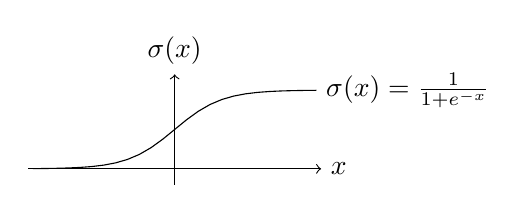
\begin{tikzpicture}[domain=-6:6,xscale=0.3]
  \draw[->] (-6.2,0) -- (6.2,0) node[right] {$x$};
  \draw[->] (0,-0.2) -- (0,1.2) node[above] {$\sigma(x)$};
  \draw plot (\x,{1 / (1 + exp(-\x))}) node[right] {$\sigma(x) = {1 \over 1 + e^{-x}}$};
\end{tikzpicture}
\caption{A sigmoidal (soft step) function.}
\label{fig:sigmoid}
\end{figure}

A number of variations for sigmoidal activation functions exist such as the 
hyperbolic tangent ($tanh$) and
the rectified linear unit \index{ReLU} (ReLU, see equation \ref{eq:ReLU}). 
They are applied either in a feed-forward or recurrent (cyclic) manner, where
the recurrent variant are forced to cope with temporal transformations to
terminate\footnote{It is possible to \textit{unfold} recurrent
networks to resemble the circular processes until a certain point, achieving
a similar effect to temporal signal transformation, see \cite{Mozer1995}.}
\cite{Schmidhuber2014}.

\begin{equation} \label{eq:ReLU}
f(x) = \begin{cases}
         0 & \text{if } x < 0 \\
	 x & \text{otherwise}
       \end{cases}
\end{equation}

Second generation neuron models typically enrich the
input signals ($x$) with a weight ($w$) as shown in \ref{eq:weightedsum}
\cite{Schmidhuber2014, Russel2007}. 
Given $n$ input neurons, the weighted sum is the value of each
input neuron ($x_i$) scaled by a weight for that individual neuron ($w_i$).
Weights allow the model to adapt the relative importance of each
input neuron by modifying their weights, thus allowing the
model to \textit{train} to a given domain \cite{Schmidhuber2014, Russel2007}.

\begin{equation} \label{eq:weightedsum}
u = w \cdot x = \sum_{i=1}^n w_i x_i
\end{equation}

For each neuron $j$ the output $x$ can be derived as shown in 
\ref{eq:weightedoutput}.

\begin{equation} \label{eq:weightedoutput}
  x_j = \sigma(u_j) = \sigma(\sum_{i=1}^n w_{i,j} x_i)
\end{equation}

\subsection{Third generation neural networks}
Constructing a network of neuron models essentially creates a non-linear
response to a given numerical vector \cite{Russel2007}.
This transformative view can be adopted to biological third generation 
\gls{SNN}, where the data being transferred are no longer vectors, but discrete
\textit{spikes} of electrical current \cite[p. 32]{Dayan2001, Eliasmith2004}.

In biological networks there is a temporal dimension to this the signals
arrive from multiple sources in parallel \cite{Eliasmith2004}.
Lapicque worked on a conductance model in 1907 that would illustrate this fact,
dubbed the \textit{integrate-and-fire} \index{neuron model!integrate-and-fire}
\index{integrate-and-fire|see {neuron model}}
model.
The model essentially integrates received current over time
to determine whether to fire
\cite{Dayan2001, Eliasmith2004}.
The Dirac ($\delta$) function \index{Dirac function}
in equation \ref{eq:dirac} shows an idealised
version of this \cite[p. 404]{Dayan2001}.
For all values it approaches 0, except when its argument is
0 where it will grow infinitely.
The total area of these `spikes' sum together to 1 over time $t$ \index{neuron spike}.

\begin{equation} \label{eq:dirac}
  \rho(t) = \int dt\ \delta(t) = 1
\end{equation}

This idealised representation is a common mathematical approximation of
a sequence of activation functions \cite{Dayan2001, Eliasmith2004},
and the foundation for the \textit{third} generation
neural networks, where the computations are understood as spikes over
time \cite{Maass1997}. \index{neuron spike} \index{spike|see {neuron spike}}
In this model the neurons receive a voltage that builds over time, until
it reaches a threshold voltage ($V_{th}$) and produces a single spike
\mbox{($\delta(t-t_n)$)}
\cite{Dayan2001, Eliasmith2004}.
In a brief period after the activation the neuron enters a period of
refraction, \index{refraction period}
where injected voltage is not accumulated, denoted by 
$\tau_{ref}$, illustrated in figure \ref{fig:spiking}
\cite[p. 82]{Eliasmith2004}.

A more realistic neuron model was developed by Hodgkin
and Huxley in 1952 dubbed the Hudgkin-Huxley model \cite{Dayan2001}.
While it is more precise than integrate-and-fire models, it is
more complex \cite[p. 195]{Dayan2001} and rarely used in simulations
\cite{Albada2018, Dayan2001, Eliasmith2015}.

\begin{figure}
\centering

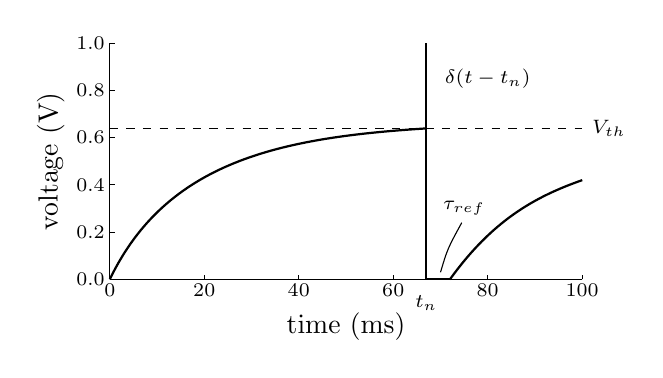
\begin{tikzpicture}[scale=3]
\pgfkeys{/pgf/number format/precision=1}
\draw (0,0) -- (2, 0);
\draw (0,0) -- (0, 1);
\foreach \i in {0,0.2,...,1}
  \draw (0,\i) -- (0.02,\i) node [left] {\scriptsize \pgfmathroundtozerofill{\i}\pgfmathresult};
\foreach \i in {0,20,...,100}
  \draw (\i/50,0) -- (\i/50,0.02) node [below] {\scriptsize \i};

\node [rotate=90] at (-0.25, 0.5) {\text{voltage (V)}};
\node at (1, -0.2) {\text{time (ms)}};

\draw [thick] (0,0) .. controls (12/50,0.50) and (36/50,0.6) .. (67/50, 0.639);
\draw [thick] (67/50,0) -- (67/50,1);
\draw [dashed] (0,0.64) -- (2,0.64) node [right] {\scriptsize $V_{th}$};
\node at (67/50, -0.1) {\scriptsize $t_n$};
\draw [thick] (67/50,0) -- ++ (0.1,0);
\node at (80/50,0.85) {\scriptsize $\delta(t-t_n)$};
\draw [thick] (72/50,0) .. controls (81/50,0.25) and (90/50,0.35) .. (2, 0.42);
\node at (75/50,0.3) {\scriptsize $\tau_{ref}$};
\draw (70/50,0.03) .. controls (71.5/50,0.13) .. (74.5/50,0.24);

\end{tikzpicture}
\caption{A model of the voltage buildup, spiking and refractory period
         of an integrate-and-fire \index{neuron model!integrate-and-fire} 
         neuron with constant current influx.}
\label{fig:spiking}
\end{figure}

Lapicque's model has been elaborated in the \textit{leaky
integrate-and-fire} (LIF) \index{neuron model!leaky-integrate-and-fire}
model, which introduces a numerical ``leak''
into the model, that acts as a type of memory \index{memory}
for the neuron integration \cite{Eliasmith2004, Eliasmith2015}.
Input voltages decays exponentially over time, meaning that the
present voltage depends more strongly on recent input voltages
\cite[p. 86]{Eliasmith2004}.
By controlling the resistance (or leak), it is possible to
control the time with which previous voltages are 'forgotten'
\cite{Eliasmith2004}.
The LIF equation is given in equation \ref{eq:lif}, where
$v$ is the membrane voltage difference between the interior
and exterior of the neuron membrane, $C(t)$ is the input current
and $\tau_{RC}$ is the membrane time constant that determines how
quickly the neuron decays to its resting state \cite{Dayan2001, Eliasmith2004}.
As soon as the voltage reaches $V_{th}$ the neuron spikes and
enters the refractory period.

\begin{equation}
  \tau_{RC}\frac{dv(t)}{dt} = -v(t) + C(t)
  \label{eq:lif}
\end{equation}

Like in the second generation neural networks, neurons
can receive input from a number of input neurons ($n$).
The connections are commonly referred to as synapses, and are similarly
weighted (see equation \ref{eq:weightedsum}), 
such that they contribute differently to the accumulated 
voltage, given by equation \ref{eq:synaptic} \cite{Dayan2001}.

\begin{equation}
  \sum_{i=1}^n{w_i\delta(t - t_i)}
  \label{eq:synaptic}
\end{equation}

\subsection{Coding spikes}
The temporal properties of the spikes convey information \cite{Dayan2001}.
Collecting spikes from a neuron over time provides a 
spike train\index{spike train} that can be decoded into numerical
values \cite{Dayan2001}.
A simple way to decode a spike train is to count the number of
spikes and divide them by the duration of the spike train, shown in
equation \ref{eq:spikerate}
\cite{Dayan2001}.

\begin{equation}
  r = {n \over T} = {1 \over T} \int_0^T \rho(t)
\label{eq:spikerate}
\end{equation}

When encoding numerical information to spikes, it is useful to 
express the spikes stochastically, such that one scalar determines
the probability that a neuron spikes over time \cite{Dayan2001}.
The firing rate can be understood as the probability that a given
neuron will fire over time \cite{Dayan2001}.
Assuming that the spikes are independent of each other, this
probability can be expressed by a distribution such as the
Poisson probability distribution\index{Poisson distribution}
\cite{Dayan2001}.
The Poisson distribution determines the probability of a number
of events occurring in an interval, given that the events are
known to happen at a fixed rate \cite{Dayan2001}.
It is defined in equation \ref{eq:poisson} where $n$ is the
number of events and $\alpha$ is the rate with which events
happen \cite{Dayan2001}.

\begin{equation}
P(n) = \alpha^n {e^{-\alpha} \over n!}
\label{eq:poisson}
\end{equation}

% TODO: Write about noise

%\subsubsection{Encoding and decoding in spiking neural networks}
%...
\begin{comment}
To align digital representations with neural spikes,
signals are encoded and decoded when entering and leaving the system
respectively \cite{Dayan2001}.
Because of the temporal nature of spiking neural networks, probability
distributions are commonly used to describe 
Given a current for background firing rates
Assuming there are $n$ inputs to a neuron with $i$ bits of information,
an encoder

\subsection{\Gls{NN}s as directed graphs}
Following the above descriptions, \gls{NN}s in both generations
can be abstracted as a directed graph: circuits of computational
units connected through	weighted, directed edges
\cite{Dayan2001, Eliasmith2004, Russel2007}.
Figure \ref{fig:nn-example} illustrates such a network.
The layered design is typical for first and second generation networks, but 
can be generalised to the third generation as well, despite their parallel
nature.
The second layer is traditionally denoted as `hidden' because it is only
stimulated indirectly \cite{Russel2007}.

\begin{figure}
\centering
\tikzset{%
  every neuron/.style={
    circle, draw, minimum size=0.5cm
  },
  neuron dots/.style={
    draw=none,
    scale=1.5,
    text height=0.3cm,
    execute at begin node=\color{black}$\vdots$
  }
}
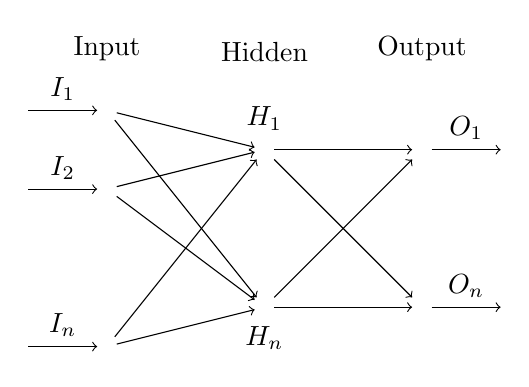
\begin{tikzpicture}{x=1.5cm, y=1.5cm}
  \foreach \m [count=\y] in {1,2,dots,n}
    \node [every neuron/.try, neuron \m/.try](input-\m) at (0, 2.5-\y) {};
  \foreach \m [count=\y] in {1, dots, n}
    \node [every neuron/.try, neuron \m/.try](hidden-\m) at (2, 2-\y) {};
  \foreach \m [count=\y] in {1, dots, n}
    \node [every neuron/.try, neuron \m/.try](output-\m) at (4, 2-\y) {};

  \foreach \l [count=\i] in {1, 2, n}
    \draw [<-] (input-\l) -- ++ (-1, 0)
      node [above, midway] {$I_{\l}$};
  \node [above] at (hidden-1.north) {$H_1$};
  \node [below] at (hidden-n.south) {$H_n$};

  \foreach \f in {1, 2, n}
    \foreach \t in {1, n}
      \draw [->] (input-\f) -- (hidden-\t);
  \foreach \f in {1, n}
    \foreach \t in {1, n}
      \draw [->] (hidden-\f) -- (output-\t);
  \foreach \l [count=\i] in {1,n}
    \draw [->] (output-\l) -- ++(1,0)
	node [above, midway] {$O_\l$};

  \foreach \l [count=\x from 0] in {Input, Hidden, Output}
    \node [align=center, above] at (\x*2,2) {\l};
\end{tikzpicture}
\caption{An example neural network with a single hidden layer.}
\label{fig:nn-example}
\end{figure}

In this representation an `input' is a stimulus vector, whose
length is equal to the number of neurons in the first layer.
Conversely, an `output' is a vector whose length
is controlled by the number of output neurons.
A \gls{NN} can then be understood as a function $f$ that 
maps an input vector to an output vector of arbitrary size
\cite{Russel2007}.

This view can be simplified as shown in figure \ref{fig:nn-composition},
such that each node is considered a function \cite{Rojas1996}.
The network is the same but the output is considered to be the sequential
composition of node functions over the input $x$.
\begin{figure}
\centering
\tikzset{%
  node/.style={
    circle, draw, minimum size=0.8cm
  }
}
\begin{tikzpicture}
  \node (input) at (-0.3,0) { $x$ };
  \node [node] (node-f) at (1.5,0) { $f$ };
  \node [node] (node-g) at (3,0) { $g$ };
  \node [node] (node-h) at (4.5,0) { $h$ };
  \node (output) at (6.5,0) { $f(g(h(x)))$ };
  \draw [->] (input) -- (node-f);
  \draw [->] (node-f) -- (node-g);
  \draw [->] (node-g) -- (node-h);
  \draw [->] (node-h) -- (output);
\end{tikzpicture}
\caption{Another representation of the network in figure
  \ref{fig:nn-example}, where each node is considered a function
and the output is derived by composing functions sequentially 
over the input.}
\label{fig:nn-composition}
\end{figure}

\section{Learning} \index{learning} \label{sec:learnin}
% TODO: http://www.cs.toronto.edu/~fritz/absps/momentum.pdf
Defining an \gls{agent} as a system that can act on previous knowledge
\cite{Russel2007}, learning in the context of an \gls{agent}
refers to ``the process of gaining
information through observation'' \cite{sep:learning-formal}.

Following the above abstraction of neural networks as computations over vectors,
``learning'' \index{learning} can be understood as the development of consistent
patterns, given the same input.
Within the \gls{ml} literature, this is commonly referred to as 
\textit{prediction}. \index{predict}
In practice this is expressed in terms of general functions or
\textit{rules} \index{rule} in a network \cite[p. 704.]{Russel2007}.

Within machine learning \gls{ml} three types of
learning exists: supervised, \index{learning!supervised}
unsupervised \index{learning!unsupervised} and reinforced.
\index{learning!reinforcement}

\textit{Supervised} learning relies on a set of expected outputs which 
the learning \gls{agent} must predict, given some input \cite{Russel2007}.
The \gls{agent} is told how `wrong' it was, so it can adapt accordingly.
This learning typically happens in a \textit{training} and \textit{testing}
phase, where the \gls{agent} is allowed to builds its internal representation
which is later tested previously unseen data \cite{Russel2007}.

\textit{Unsupervised} learning asks the \gls{agent} to learn without
having any idea of error margin \cite{Russel2007}.
Rather, the \gls{agent} is asked to \textit{explore} a domain in search of
patterns, which then form the basis for future predictions or classifications
\cite{Russel2007}.

\textit{Reinforced} learning reinforces the \gls{agent} through
rewards and discourages it through punishments \cite{Russel2007}.
Contrary to supervised learning the rewards and punishments are not
instructing the agent on what the output should be, but rather how well
it performed the task, leaving the \gls{agent} to infer rules or
behaviours by itself \cite[p. 873]{Russel2007}.

The process of learning can either be \textit{inductive}
\index{learning!induction}
or \textit{deductive} \index{learning!deduction} \cite[p. 704]{Russel2007}.
The latter requires a basis in rule-based systems from which new knowledge can
be deduced, while the former requires a measurement of success \cite[p. 705]{Russel2007}.
Such a measurement is typically referred to as the \textit{error} or \textit{loss}
function,\index{loss function}\index{error function|see {loss function}}
because it shows how much the prediction deviated from the expectation (goal)
\cite{Russel2007}.

Learning within neural networks have shown to be possible within all three
types of learning \cite{Schmidhuber2014, Russel2007}, but deduction is rarely
seen in the \gls{NN} literature, because it is cumbersome to express neural
networks through logic transformations \cite{Pearl2018}.
%TODO: Check citation; write about Eliasmith and DTU logics guy
Because of its simplicity and widespread use, this thesis will focus on supervised
inductive learning.

\subsection{Errors in learning}
It is worth noting that \gls{NN}s may learn \index{learn}
rules \index{rule} that are not optimal \cite{Russel2007}.
This can happen in one of two ways: either the
network is structurally incapable of learning the domain, 
or the learned rule is incorrect \cite{Russel2007, Eliasmith2015}.

A \gls{NN} is limited in complexity by its number of nodes,
because one neuron is only capable of describing a limited
outcome \cite{Dayan2001, Russel2007}.
This is sufficient to model a linear correlation, but insufficient
to explain, complex dependencies by itself.
Such a structural limit cannot be solved by any other means
than augmenting the network \cite{Russel2007}.

Provided that the network is sufficiently complex, the 
learned rules can still be incorrect if the data, on which
the network bases its predictions, fails to capture the 
expectations of the trainer.
In other words the data can fail to represent the problem 
correctly \cite{Russel2007}.
To avoid this, it is customary to only train the network
on a part of the available data, only to test it on 
the remaining data \cite{Russel2007, Schmidhuber2014}.
The limits between data for training and data for testing
are not agreed upon, but a 80\%/20\% split seems to be
the default \cite{Russel2007, Schmidhuber2014}.

\subsection{Backpropagation}
Returning to the analogy of neural networks as functions
over vectors, learning can be understood as a search for
the optimal weight configuration, such that prediction
errors are minimised \cite{Rumelhart1988}.
Thus the network weights constitutes the search space, 
and the loss function \index{loss function}
is the subject of the optimisation \cite{Russel2007}.

The loss function to minimize for a supervised network
is described in equation \ref{eq:bp-loss},
where the actual output $x$ is compared to the 
target (desired) output $t$, for all output neurons $n$
\cite{Russel2007}.

\begin{equation}
  E = {1 \over 2} \sum_{i=1}^n |x_i - t_i|^2
  \label{eq:bp-loss}
\end{equation}

For feedforward networks this calculation happens
through the sequential application of the weighted activation
functions in each layer, such that the value of $x_i$
depends on the value from the connected previous neurons.
For second generation neural networks this makes the
error function continuous and differentiable,
such that the gradient of $E$ with respect to the layer weights
($w_1 \cdots w_l$) can be found, and the weights can be iteratively
adjust \cite{Rojas1996}, as shown in equation \ref{eq:bp-derivation}.

\begin{equation}
  \Delta E = (
    {\partial E \over \partial w_1}, 
    {\partial E \over \partial w_2},
    \cdots, 
    {\partial E \over \partial w_l}
  )
  \label{eq:bp-derivation}
\end{equation}

Incrementally, each weight can be updated as in equation \ref{eq:bp-update},
where $\gamma$ is a factor that controls the speed with which the weights
are corrected (learning rate). \index{learning rate}

\begin{equation}
  \Delta w_i = -\gamma {\partial E \over \partial w_i}
  \label{eq:bp-update}
\end{equation}

This technique is referred to as gradient descent, because the weights
traverse the gradient towards a minimum \cite{Russel2007}.
Whether that minimum is local or not is uncertain, why it is
important to note that this technique is vulnerable to 
local protuberances \cite{Rojas1996, Russel2007}.
The learning rate exists to avoid ``shooting over'' optimal points, and
several techniques have been invented to circumvent the problem of 
local minima\footnote{Two examples are to give the learning rate a
  ``momentum'', that alters the learning rate based on the previous 
  success in minimising the loss function, 
  or to assign individual learning rates for each weight
  \cite{Schmidhuber2014}. Many more techniques exist, but they will
  not be covered here.
} \cite{Russel2007}.

Because the computation of the output layer is the result of the
previous layer,

Backpropagation, as it was invented by
\textcite{Rumelhart1988}, is an algorithm that ``looks for the minimum
of the error function in weight space using the method
of gradient descent'' \cite[p. 151]{Rojas1996}.
The idea is based on the application of the 

For feedforward networks By deriving the 
searches for optima by calculating the negative
gradients of this loss function \cite{Rumelhart1988}.
In a neural network the error is calculated at the output
layer and `pushed' backwards, so as to incrementally 
correct the network weights, such that .

% TODO: Write in

%\subsubsection{Auto-differentiation}
% TODO: Write about autodiff

%\section{Connection-set algebra} \label{sec:CSA}

\section{The biological brain}
\subsection{Plasticity in the brain}
\subsection{REF model} \label{sec:ref}

\section{Neuromorphic computing}
\end{comment}
\end{document}
